\documentclass[11pt]{article}
\usepackage{amsmath, amssymb}
\usepackage{graphicx}
\usepackage{geometry}
\usepackage{booktabs}
\usepackage{hyperref}
\usepackage{subfigure}  
\geometry{a4paper, margin=1in}

\title{Modeling Analysis Report on Survival of Allogeneic Hematopoietic Cell Transplantation (HCT) Patients}
\author{}
\date{}

\begin{document}

\maketitle

\section*{1. Introduction}
Survival analysis is a crucial branch of statistics that focuses on analyzing the time until an event of interest occurs. It is particularly important in medical research, such as evaluating the survival time of cancer patients or the time to complications after transplantation. Survival datasets typically contain censored observations, especially right-censored data, meaning that the event of interest (e.g., death) has not occurred by the end of the study for some individuals, making their exact survival times unknown.

\noindent This study utilizes a dataset of patients who underwent allogeneic hematopoietic cell transplantation (HCT). The objective is to evaluate and compare the predictive performance (C-index) of various models and identify key factors that influence patient survival using feature importance analysis.

\section*{2. Dataset Overview and Preprocessing}
\subsection*{2.1 Dataset Description}
1. The dataset comprises 28,800 samples and 60 variables, including:
\begin{itemize}
  \item 2 target variables: \texttt{efs} (event occurrence) and \texttt{efs\_time} (event time),
  \item 1 unique patient ID,
  \item 57 feature variables.
\end{itemize}

\noindent 2. Only 7 features are completely free of missing values. 8 features have more than 20\% missing data, with the highest missing rate reaching 58\%. Most features with fewer than 20 unique values tend to be categorical, which requires proper encoding methods.

\noindent 3. Regarding censoring, 46\% (13,268) of patients are right-censored, indicating they were still alive at the time of data cutoff. The distribution of censored data is skewed to the right. Thus, modeling must appropriately handle censored cases.

\begin{figure}
    \centering
    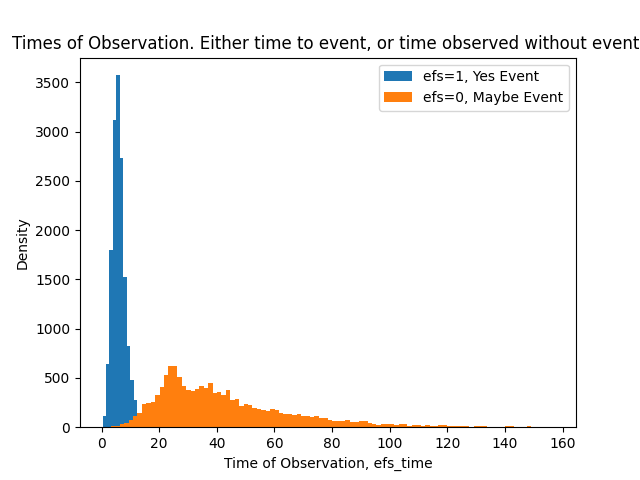
\includegraphics[width=0.75\linewidth]{03-event-density.png}
    \caption{Distribution Plot of Censored Events}
    \label{fig:enter-label}
\end{figure}

\subsection*{2.2 Preprocessing Steps}
\begin{enumerate}
  \item \textbf{Feature Removal:} Drop features with missing values exceeding 20\%.
  \item \textbf{Missing Value Imputation:} Fill remaining missing values with \texttt{NA} to facilitate model compatibility.
  \item \textbf{Categorical Encoding:} Encode features with fewer than 20 unique values as Categorical features to accommodate model training.
\end{enumerate}

\section*{3. Modeling Approaches}
The primary goal is to predict survival probability based on \texttt{efs} and \texttt{efs\_time}, while accounting for right-censoring. Two baseline survival models are used: the Kaplan-Meier estimator and Cox proportional hazards model. These are then integrated with XGBoost, CatBoost, and LightGBM to construct five hybrid models.

\subsection*{3.1 Kaplan-Meier Estimator}
The Kaplan-Meier (KM) estimator is a non-parametric method for estimating survival probability:
\[
S(t) = \prod_{t_i \leq t} \left(1 - \frac{d_i}{n_i}\right)
\]
where $d_i$ is the number of events at time $t_i$, and $n_i$ is the number of individuals at risk just before $t_i$. \\
\noindent In the context of this dataset:

\begin{enumerate}
  \item Sort the samples in ascending order based on event time. Handle censored data appropriately: censoring time affects only the risk set but not the event count.
  
  \item For each time point $t_i$:
  \begin{itemize}
    \item Compute $d_i$, the number of events (e.g., deaths) occurring at time $t_i$, and $n_i$, the number of individuals at risk just prior to $t_i$.
    \item Update the survival probability as:
    \[
    S(t_i) = S(t_{i-1}) \times \left(1 - \frac{d_i}{n_i}\right)
    \]
  \end{itemize}
  
  \item After iterating through all event times, assign each sample its corresponding survival probability $S(t)$, effectively merging the \texttt{efs} (event indicator) and \texttt{efs\_time} (event time) variables into a single target variable $S(t)$, which can be used as the target for predictive modeling.
\end{enumerate}

\noindent The algorithm handles censoring by only including uncensored cases in the calculation of $d_i$, but counting censored cases in $n_i$ up to the time of censoring.

\subsection*{3.2 Cox Proportional Hazards Model}
The Cox model assumes a hazard function of the form:
\[
h(t|X) = h_0(t) \exp(\beta^T X)
\]
where $h_0(t)$ is the baseline hazard and $\beta$ represents feature coefficients. Parameters are estimated via partial likelihood:
\[
L(\beta) = \prod_{i=1}^{n} \left[\frac{\exp(\beta^T X_i)}{\sum_{j \in R(t_i)} \exp(\beta^T X_j)}\right]^{\delta_i}
\]
with $R(t_i)$ being the risk set at $t_i$, and $\delta_i = 1$ if the event occurred.

\subsection*{3.3 Hybrid Models with Gradient Boosting}
We construct five models by combining KM or Cox-based labels with gradient boosting frameworks. \\

\noindent In Kaplan-Meier-type models, the survival probability $S(t)$ is estimated based on the \texttt{efs} (event indicator) and \texttt{efs\_time} (event time). Then, $S(t)$ is used as the target variable, while the feature variables are used as predictors. Three gradient boosting models—XGBoost, CatBoost, and LightGBM—are trained to fit the relationship between features and survival probability. Finally, the trained models are used to predict survival probabilities on the test set. \\

\noindent In Cox-type models, the partial likelihood function of the Cox proportional hazards model is used as the loss function. The models learn and optimize based on the feature variables to find the best model fit. In this category, both XGBoost and CatBoost are employed to perform survival modeling and optimization. \\

\noindent Below is a brief introduction to the gradient boosting methods used:


\subsubsection*{XGBoost}
XGBoost is an efficient implementation of gradient boosted decision trees (GBDT), optimizing:
\[
L = \sum_{i=1}^n L(y_i, \hat{y}_i) + \sum_{k=1}^K \Omega(f_k)
\]
with regularization $\Omega(f_k) = \gamma T + \frac{1}{2} \lambda \|w\|^2$ to prevent overfitting.

\subsubsection*{CatBoost}
CatBoost is optimized for categorical data. Its innovations include:
\begin{itemize}
  \item \textbf{Target Statistics Encoding:} Encodes categorical features using historical label statistics to avoid leakage.
  \item \textbf{Ordered Boosting:} Ensures unbiased gradient estimation.
  \item \textbf{Symmetric Trees:} Improves prediction consistency and efficiency.
\end{itemize}

\subsubsection*{LightGBM}
LightGBM enhances speed and memory efficiency via:
\begin{itemize}
  \item Histogram-based training,
  \item Gradient-based One-Side Sampling (GOSS),
  \item Exclusive Feature Bundling (EFB),
  \item Leaf-wise tree growth.
\end{itemize}

\section*{4. Results and Comparison}
\subsection*{4.1 Evaluation Metric: Concordance Index}
Due to the specific characteristics of survival analysis datasets, the predictive performance of models is evaluated using the Concordance Index (C-index). The C-index is a commonly used metric in survival analysis that measures the concordance between predicted risks and actual survival times. It is defined as the proportion of all comparable pairs of samples in which the individual with a higher predicted risk experiences the event earlier. The mathematical expression is as follows:
\[
\text{C-index} = \frac{\sum_{i,j} I(T_i < T_j \land \hat{h}_i > \hat{h}_j \land \delta_i = 1)}{\sum_{i,j} I(T_i < T_j \land \delta_i = 1)}
\]
\noindent
Where: \\
\begin{itemize}
    \item $T_i, T_j$ represent the actual event times (or censoring times).
    \item $\hat{h}^i, \hat{h}^j$ are the predicted risk scores by the model.
    \item $\delta_i = 1$ indicates that individual $i$ experienced the event (i.e., was not censored).
\end{itemize}

\noindent A value of 0.5 implies random prediction, while 1.0 indicates perfect accuracy.

\subsection*{4.2 Performance Results}
Based on the algorithm descriptions above, five models were trained and fitted to predict survival, with their corresponding C-index results shown in the table below. \\
\noindent From the results, it can be observed that the C-index values of the five models are quite close, ranging from 0.6733 to 0.6757. Among them, the XGB-Cox model performed the best. XGBoost demonstrated stable performance under both the Kaplan-Meier and Cox frameworks, achieving C-index values of 0.6751 and 0.6757, respectively. CatBoost and LightGBM showed slightly more fluctuation in performance, especially under the Cox framework, where they performed somewhat less effectively.

\begin{table}[h!]
\centering
\caption{Model Performance (C-index)}
\begin{tabular}{ll}
\toprule
Model & C-index \\
\midrule
XGB-Kap Model & 0.6751 \\
CatBoost-Kap Model & 0.6744 \\
LightGBM-Kap Model & 0.6745 \\
XGB-Cox Model & \textbf{0.6757} \\
CatBoost-Cox Model & 0.6733 \\
\bottomrule
\end{tabular}
\end{table}

\subsection*{4.3 Feature Importance Analysis}
The top important features in different models are shown below. We can get these key findings from feature importance analysis:

\begin{itemize}
  \item \textbf{XGB-Cox:} Top features include \texttt{conditioning\_intensity}, \texttt{dri\_score}, and \texttt{comorbidity\_score}.
  \item \textbf{CatBoost-Kap:} \texttt{dri\_score} is most important, followed by \texttt{conditioning\_intensity} and \texttt{comorbidity\_score}.
  \item \textbf{LightGBM-Kap:} \texttt{donor\_age}, \texttt{age\_at\_hct}, and \texttt{dri\_score} dominate.
\end{itemize}

\begin{figure}[htbp]
    \centering
    \subfigure[XGB Kaplan Top Importance Features]{
        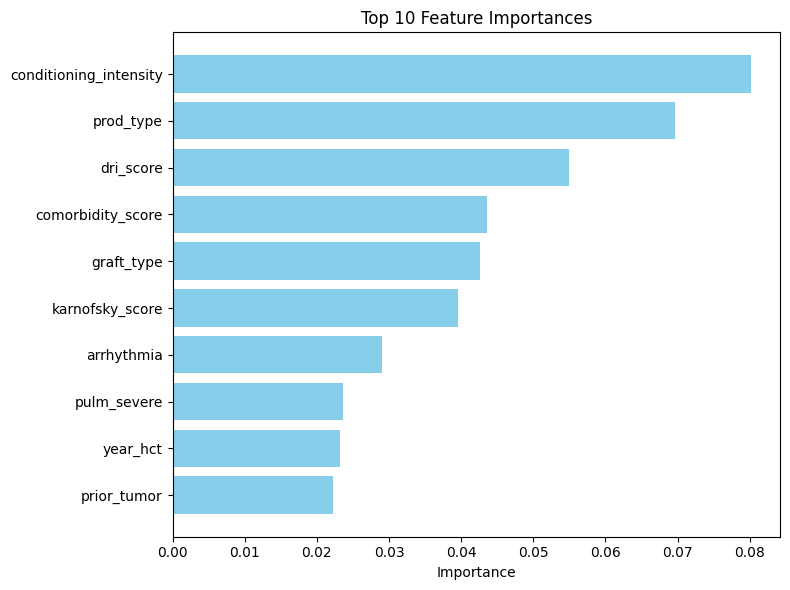
\includegraphics[width=0.45\textwidth]{01_xgb_Kaplan_Top10_feature_importance.png}
        \label{fig:image1} }
    \subfigure[CatBoost Kaplan Top Importance Features]{
        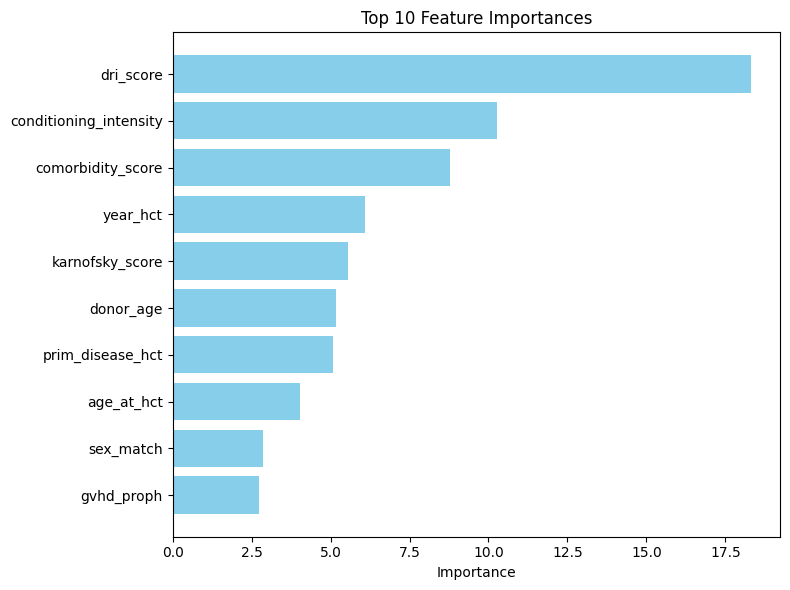
\includegraphics[width=0.45\textwidth]{02_cat_Kaplan_Top10_feature_importance.png}
        \label{fig:image2} }
    \label{fig:twoimages}
\end{figure}

\begin{figure}[htbp]
    \centering
    \subfigure[LightGBM Kaplan Top Importance Features]{
        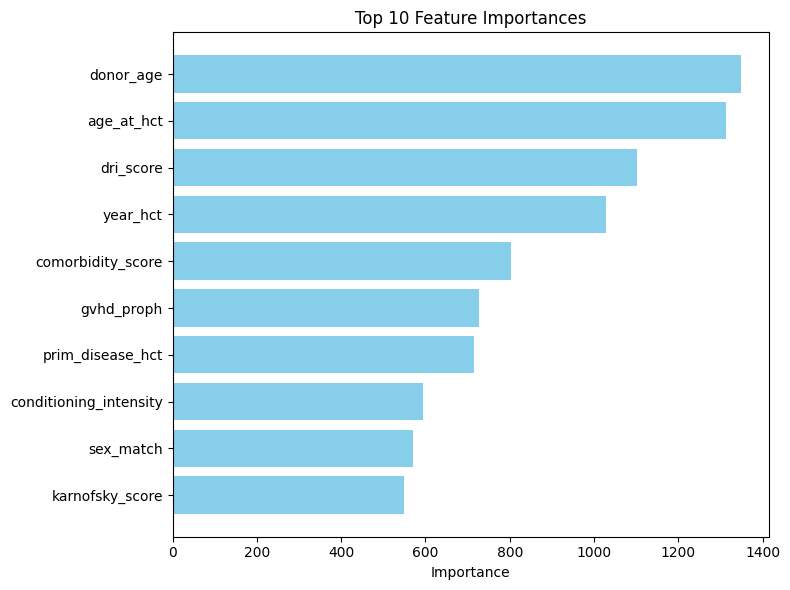
\includegraphics[width=0.3\textwidth]{03_LightGBM_Kaplan_Top10_feature_importance.png}
        \label{fig:image1}
    }
    \subfigure[XGB Cox Top Importance Features]{
        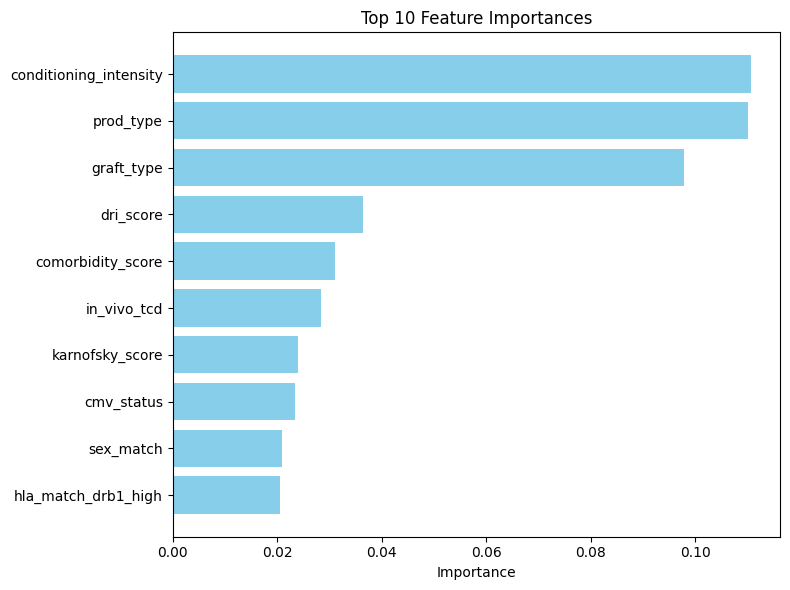
\includegraphics[width=0.3\textwidth]{04_XGB_Cox_Top10_feature_importance.png}
        \label{fig:image2}
    }
    \subfigure[Cat Cox Top Importance Features]{
        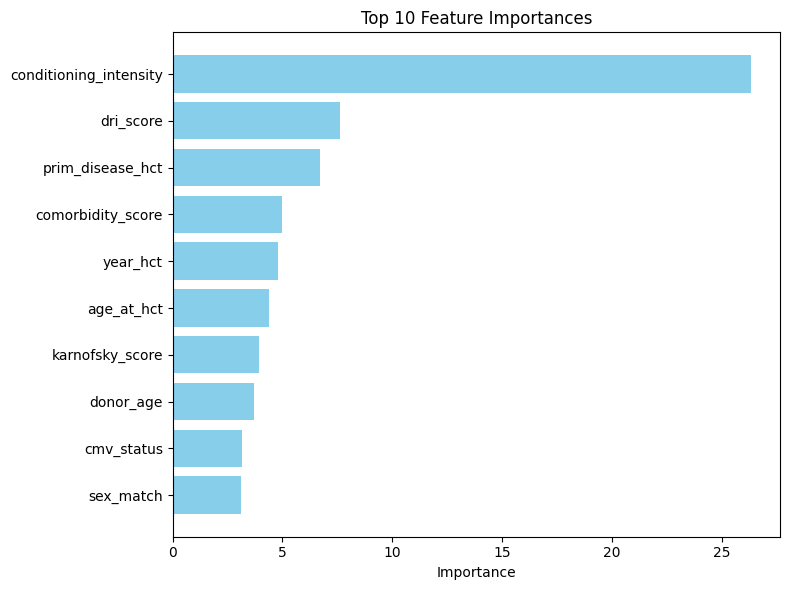
\includegraphics[width=0.3\textwidth]{05_Cat_Cox_Top10_feature_importance.png}
        \label{fig:image3}
    }
    \caption{Top Importance Features}
    \label{fig:threeimages}
\end{figure}


\noindent Based on the feature importance rankings across the five models, the key factors affecting the survival probability of HCT patients include:
\begin{enumerate}
    \item \textbf{Disease Risk Index (dri\_score)}: Ranked highly in all models, indicating that disease risk is one of the most critical factors influencing patient survival. Therefore, patients with high-risk diseases (e.g., AML, ALL) may require more intensive treatment strategies.
    
    \item \textbf{Conditioning Intensity (conditioning\_intensity)}: Has a significant impact on survival probability, especially ranking high in Kaplan-Meier-based models. Patients with different risk profiles may require different types of conditioning regimens. Myeloablative conditioning (MAC) and reduced-intensity conditioning (RIC) may be suitable for different risk groups.
    
    \item \textbf{Comorbidity Score (comorbidity\_score)}: Reflects the overall health condition of the patient and is closely associated with survival outcomes.
    
    \item \textbf{Year of Transplantation (year\_hct)}: May reflect the influence of advances in medical technologies on survival rates.
    
    \item \textbf{Performance Status Score (karnofsky\_score)}: The physical performance of the patient plays a critical role in determining survival probability.
    
    \item \textbf{Age-related Factors (age\_at\_hct, donor\_age)}: The ages of both the patient and the donor are especially important in the LightGBM model, suggesting that age significantly affects transplant outcomes. Younger patients and younger donors may be associated with better prognosis.
\end{enumerate}

\section*{5. Conclusion}
This study evaluated five models for survival prediction of HCT patients, using Kaplan-Meier and Cox models in combination with XGBoost, CatBoost, and LightGBM. The XGB-Cox model achieved the highest C-index (0.6757), suggesting superior performance in handling censored data and capturing complex feature interactions.\\


\noindent Moreover, consistent patterns in feature importance underscore the critical role of clinical factors such as disease risk, conditioning regimen, comorbidities, and patient/donor age in predicting post-transplant survival. These insights can inform clinical decision-making and personalized treatment planning.For example, particular attention should be paid to the patient's disease risk and comorbidity status before transplantation, while optimizing the conditioning regimen to improve survival rates.


\end{document}
